%!TEX root = ../thesis.tex
%*******************************************************************************
%****************************** Third Chapter **********************************
%*******************************************************************************
\chapter{Summary and future research} \label{sec:sum}

\ifpdf
    \graphicspath{{Chapter6/Figs/Raster/}{Chapter6/Figs/PDF/}{Chapter6/Figs/}}
\else
    \graphicspath{{Chapter6/Figs/Vector/}{Chapter6/Figs/}}
\fi

The dogmatic view that organisms are predetermined by their genetic code has been shattered by the discovery of epigenetic factors, including DNA methylation, histone modifications, and small non-coding RNA sequences. DNA methylation has been the topic of this thesis, which is involved in important biological processes, including gene regulation, imprinting, X-chromosome inactivation, and the repression of retroviruses. Single-cell DNA methylation profiling protocols are promising for studying DNA methylation at a single-cell resolution and for understanding differences between cells. However, current protocols are limited by incomplete CpG coverage and high-levels of technical noise, which renders downstream analyses challenging.

In this thesis, we presented computational methods for the analysis of single-cell methylation data. In \cref{sec:pro}, we described computational methods for the analysis DNA methylation in single cells, which we developed jointly with seminal single-cell profiling protocols. We described scBS-seq, a protocol (\Cref{sec:bs}) for genome-wide profiling of DNA methylation in single cells, and a statistical model for estimating methylation heterogeneity in different genomic contexts. We further presented scM\&T-seq, a protocol (\Cref{sec:mt}) for parallel profiling of DNA methylation and gene expression in the same cell, and methods for estimating associations between the methylome and transcriptome. By identifying both previously known and novel regulatory associations between DNA methylation and gene expression, we demonstrated that scM\&T-seq is a powerful approach for investigating the poorly understood relationship between transcriptional and epigenetic heterogeneity in single cells.

The low CpG coverage of single-cell methylation profiles renders genome-wide analyses challenging. Hence, methods for imputing methylation profiles are critical. In \cref{sec:dcpg}, we described DeepCpG, a computational approach based on deep neural networks for predicting methylation states in single cells. Unlike previous methods, DeepCpG is based on a modular architecture to learn informative features in a data-driven manner and leverages information from multiple cells. By evaluating DeepCpG on single-cell methylation data from five cell types generated using alternative sequencing protocols, we demonstrated that DeepCpG yields substantially more accurate predictions than previous methods and is widely applicable.

In \cref{sec:dcpg_ana}, we described approaches for interpreting the learned parameters of DeepCpG. By interpreting the filters of the first convolutional layer as sequence motifs, we have shown that DeepCpG learns both previously known and potentially new motifs that are associated with DNA methylation states. We have further developed a scoring approach to discern motifs that are either primarily associated with cell-to-cell variance or mean DNA methylation levels. Third, we have presented a gradient-based approach to efficiently estimate the effect of single nucleotide mutations on DNA methylation, and have shown that estimated effects are significantly increased for experimentally validated mQTLs.

There are many open leads for future research. DeepCpG does not estimate predictive uncertainty, which makes it hard to decide if predictions are accurate enough for a particular downstream analysis. Extending DeepCpG to estimate predictive uncertainty is one important future research direction. Inspiration might be drawn from Bayesian neural networks~\citep{neal_bayesian_2012}, which are, however, limited by high computational costs. Recently, \citet{gal_dropout_2015-1} described the use of dropout for performing approximate Bayesian inference and representing uncertainty in a computationally efficient manner. This approach is straightforward to implement in DeepCpG since it already uses dropout for regularization.

Another important avenue of future research is to further improve the interpretability of DeepCpG. We have shown that the filters of the first convolutional layer of the DeepCpG DNA module can be interpreted as sequence motifs, and hence DeepCpG be used for motif discovery. It is interesting to also analyse higher-level convolutional features, which may reveal more complex sequence patterns that are composed of elementary motifs. Higher-level features can be visualized, for example, by activation maximization~\citep{mahendran_visualizing_2015}, a technique that uses the gradient signal to find the model inputs that maximally activate a certain feature. An alternative way to improve the interpretability is attention~\citep{cho_describing_2015}. Attention mechanisms have been used to identify the most salient input features, such as regions in an image that are most relevant for a certain prediction task~\citep{cho_describing_2015,xu_show_2015,sharma_action_2015}. In particular soft-attention is straightforward to implement in DeepCpG and provides the potential to better understand which regions in the DNA sequence window or which cells are most relevant for predicting DNA methylation.

\begin{figure}[htbp!]
\centering
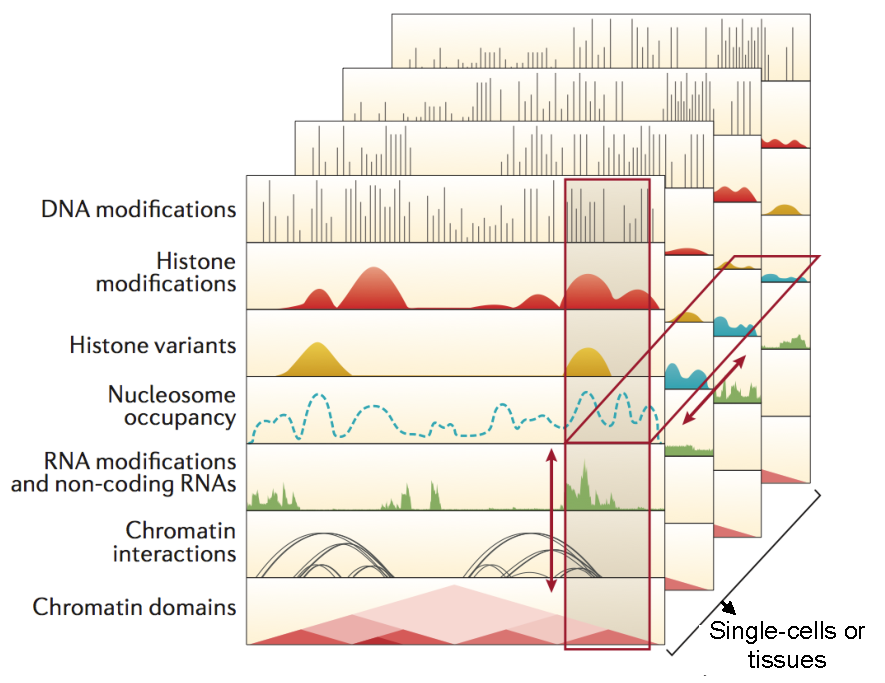
\includegraphics[width=0.9\textwidth]{multi}
\caption[Imputation of multiple molecular layers in multiple cells.]{Imputation of multiple molecular layers in multiple cells. Missing layers are imputed by sharing information both between molecular layers and between cells. Source: \citet{stricker_profiles_2016}.}
\label{fig:sum_multi}
\end{figure}

DeepCpG predicts methylation states independently for each CpG site and cell. Extending DeepCpG to take dependencies between its predictions into account is likely to further improve prediction accuracy. Appealing for this purpose are conditional generative models, including generative recurrent neural networks~\citep{graves_generating_2013, chung_recurrent_2015}, pixel convolutional neural networks~\citep{oord_pixel_2016,kalchbrenner_neural_2016,oord_wavenet:_2016}, and restricted Boltzmann machines~\citep{sutskever_recurrent_2009,boulanger-lewandowski_modeling_2012,boulanger-lewandowski_high-dimensional_2013,bayer_learning_2014}. These models have been successfully used for generating handwriting, natural text, and audio sequences, and can be adapted to also generate a sequence of methylation states conditioned on partially observed methylation states and the DNA sequence.

DeepCpG is trained using information from the DNA sequence and incomplete DNA methylation profiles. An important extension of DeepCpG is to integrate additional data modalities profiled in the same cells, for example gene expression and copy number variations. These data modalities can be integrated by additional modules that are specific for each modality. Alternatively, data modalities can be processed jointly by representing them analogously to the colour channels of a multi-dimensional image tensor.

DeepCpG has been designed for imputing a single data modality (DNA methylation) in multiple cells from one or more input data modalities. More general are models for imputing multiple data modalities in multiple cells (\Cref{fig:sum_multi}). These models would be more broadly applicable to sets of cells that were profiled using different parallel profiling protocols.  In this settings, some data modalities, e.g. DNA methylation and gene expression, might be available in a subset of cells but missing or only partially be available in a subset of cells that was processed using a different protocol, e.g. for profiling DNA accessibility and histone modifications. Missing data modalities can be imputed by sharing information both between data modalities and between cells. Based on this idea, \citet{ernst_large-scale_2015} proposed an ensemble of regression trees for imputing multiple epigenomic profiles in bulk populations of cells. Appealing deep neural network architectures for learning from multi-modal data are, for example, Boltzmann machines~\citep{srivastava_multimodal_2012}, autoencoders~\citep{chandar_correlational_2015,rajendran_bridge_2015}, variational autoencoders~\citep{pandey_variational_2016,suzuki_joint_2016,serban_multi-modal_2016}, and deep canonical correlation analysis~\citep{andrew_deep_2013,benton_deep_2017}. These architectures exchange information between data modalities by shared latent representations, which are inferred from the observed data and used to impute missing data.

Multi-modal latent variable models are also well suited for analysing the factors of variations that underlie epigenetic data. Inferring latent variables that are either shared across or specific to individual cells and molecular layers can help to better characterize cells and molecular layers as well as their relationships. Inferring latent variables of individual cells enables clustering cells, detecting outlier cells, and interpreting the type and state of cells. Inferring latent variables that are shared across and specific to data modalities enables investigating the relationships between molecular layers, for example associations between gene expression and DNA methylation. While latent variable models are promising for imputing and understanding multi-modal epigenetic data, they are often limited by high computational costs. Developing models that are computational efficient is critical for genome-wide analyses of large datasets and practical applications. Another challenge is the integration data that are profiled at different scales, for example per base pair, per CpG sites, or per gene. Finally, methods must be user-friendly and easy to use by non-experts.
